\section{Bootscanning}
\label{sct_bootscanning}

Bootscanning is a technique for finding recombination breakpoints in a
sequence. It involves aligning the sequence of interest (called \emph{query} or
\emph{reference}) with related sequences (including the putative recombinant's
parents) and computing phylogenies locally over the alignment. Recombination is
expected to cause changes in topology.  The tasks involved are shown below:
\begin{enumerate}
\item align the sequences $\rightarrow$ multiple alignment
\item slice the multiple alignment $\rightarrow$ slices
\item build a tree for each slice $\rightarrow$ trees
\item extract distance from query to other sequences (each tree) $\rightarrow$ tabular data
\item plot data $\rightarrow$ graphics
\end{enumerate}
The distribution contains a script, \texttt{src/bootscan.sh}, that performs the whole process. Here is an example run:
\begin{verbatim}
$ bootscan.sh HRV_3UTR.dna HRV-93 CL073908
\end{verbatim}
where \texttt{HRV\_3UTR.dna} is a FastA file of (unaligned) sequences, \texttt{HRV-93} is the outgroup, and \texttt{CL073908} is the query.  Here is the result:

\begin{centering}
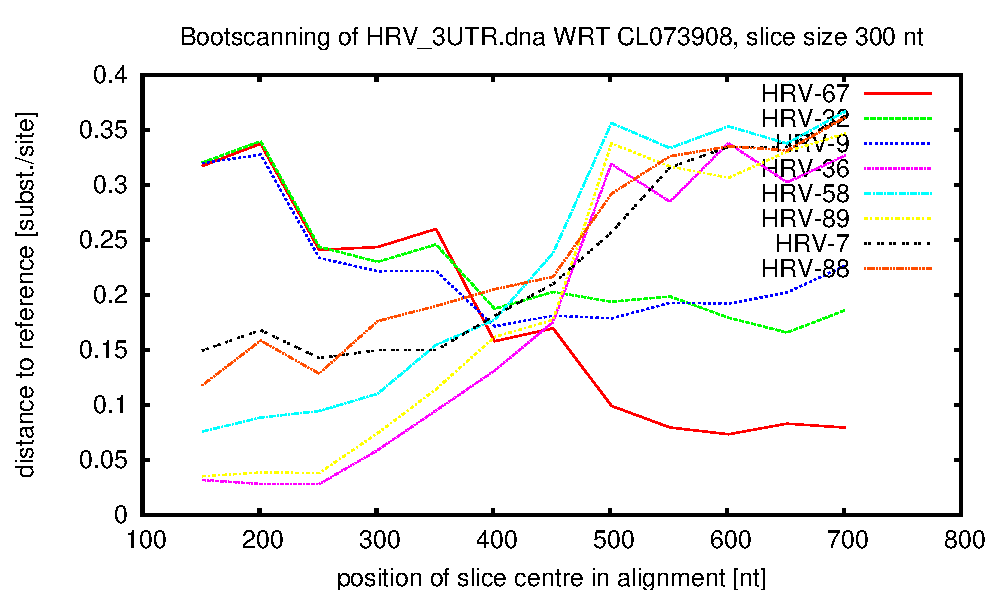
\includegraphics[scale=0.7]{bootscan_1.pdf}
\end{centering}

\smallskip{}
\noindent{}until position 450 or so, the query sequence's nearest relatives (in
terms of substitutions/site) are \texttt{HRV-36} and \texttt{HRV-89}. After
that point, it is \texttt{HRV-67}. This suggests that there is a recombination
breakpoint near position 450.

The script uses \reroot{} to reroot the trees on the outgroup, \clade{} and
\labels{} to get the labels of the ingroup, \distance{} to extract the distance
between the query and the other sequences, as well as the usual \texttt{sed}, \texttt{grep}, etc. The plot is done with gnuplot.
